\documentclass[a4paper,12pt]{report}
\usepackage{titlesec}
\usepackage{amssymb} 
\usepackage{graphicx} 
\usepackage{geometry}
\usepackage{longtable}
\geometry{a4paper,left=25mm,right=25mm,top=30mm,bottom=30mm}
\usepackage{float}
\usepackage{cite}
\usepackage{titlesec}
\titleformat{\chapter}[display]
  {\normalfont\huge\bfseries\centering}
  {\chaptertitlename\ \thechapter}{20pt}{\Huge}

\begin{document}
\thispagestyle{empty}
\begin{center}
 \huge{\textsc{Optimisation of Antenna Design using Machine Learning}}
\end{center}
\vspace{0.25cm}
\begin{center}
 \normalsize{\textit{Project report submitted in partial fulfillment of the requirement for the degree of}}
\end{center}
\begin{center}
\large{Bachelor of Technology }
\end{center}
\vspace{0.5cm}
\begin{center}
 \normalsize{Submitted by}
\end{center}
\vspace{0.5cm}
\begin{center}
 \large{Akshat Punia (2010110062)}\\
  \vspace{0.25cm}
 And\\
 \vspace{0.25cm}
 \large{Sarvesh Sankaran (2010110569)}
\end{center}
 \vspace{0.25cm}
\begin{center}
 \large{Under Supervision of}
\end{center}
\vspace{0.25cm}
\begin{center}
 \large{Jitendra Prajapati}\\
 \large{Department of Electrical Engineering}\\
 \vspace{0.25cm}
\end{center}
\begin{figure}[htbp]
	\centering
		
\includegraphics[width=4in]{logonew.jpg}	
\end{figure}
\vspace{0.25cm}
\begin{center}
\large{\textbf{Department of Electrical Engineering}}\\
\large{\textbf{School of Engineering}}\\
\large{\textbf{Shiv Nadar Institution of Eminence}}\\
\vspace{0.25cm}
(December 2023)
\end{center}
\pagebreak
\begin{center}
\huge{\textsc{Candidate Declaration}}
\vspace{1cm}
\end{center}
We hereby declare that the thesis entitled “Optimisation of Antenna Design Using Machine Learning” submitted for the B. Tech. degree program. This thesis has been written in our own words. We have adequately cited and referenced the original sources.
\vspace{2cm}\\
\begin{minipage}{4.5cm}
Akshat Punia\\
(2010110062)
\end{minipage}
\hfill
\begin{minipage}{4.5cm}
Sarvesh Sankaran\\
(2010110569)
\end{minipage}
\pagebreak
\begin{center}
\huge{\textsc{Certificate}}
\vspace{1cm}
\end{center}
It is certified that the work contained in the project report titled “Optimisation of Antenna Design Using Machine Learning,” by “Akshat Punia” has been carried out under my supervision and that this work has not been submitted elsewhere for a degree.
\vspace{2cm}\\
\begin{minipage}{7cm}
Jitendra Prajapati\\
Dept. of Electrical Engineering\\
School of Engineering\\
Shiv Nadar Institution of Eminence\\
Date: 28/11/2023 
\end{minipage}
\pagebreak
\begin{center}
\huge{\textsc{Certificate}}
\vspace{1cm}
\end{center}
It is certified that the work contained in the project report titled “Optimisation of Antenna Design Using Machine Learning,” by “Sarvesh Sankaran” has been carried out under my supervision and that this work has not been submitted elsewhere for a degree.
\vspace{2cm}\\
\begin{minipage}{7cm}
Jitendra Prajapati\\
Dept. of Electrical Engineering\\
School of Engineering\\
Shiv Nadar Institution of Eminence\\
Date: 28/11/2023 
\end{minipage}
\pagebreak
\begin{center}
\huge{\textsc{Abstract}}
\end{center}
For electromagnetic design problems, various computation methods have
been applied and have shown promising results. However, these
algorithms often entail substantial computational expenses due to the
demanding nature of electromagnetic simulations. As a consequence,
direct application of these algorithms for optimization can result in
extensive time requirements, sometimes spanning weeks. This drawback
restricts their applicability within numerous real-world industrial scenarios.
This project aims to address this limitation by exploring and implementing
machine learning techniques. The objective is to facilitate simulation-
optimized antenna design within a feasible timeframe. This will be achieved
through the utilization of a simulated dataset, encompassing various
samples with distinct design parameters while maintaining a consistent
substrate material and thickness. The dataset will be generated via the
electromagnetic simulator CST Microwave Studio.
\pagebreak
\tableofcontents
\pagebreak
\listoffigures
\pagebreak
\listoftables
\pagebreak




\chapter{Introduction}
\label{chap:introduction}

\section{Background and Motivation}
Electromagnetic design problems have been addressed using various computational methods, which have demonstrated promising results. However, these algorithms often come with substantial computational expenses due to the demanding nature of electromagnetic simulations. Consequently, the direct application of these algorithms for optimization can lead to extensive time requirements, sometimes spanning weeks or even longer. Such a drawback significantly limits their applicability within numerous real-world industrial scenarios, where rapid design iterations are crucial for competitiveness and efficiency.

\section{Research Objective}
This project seeks to overcome this limitation by exploring and implementing machine learning techniques in the domain of antenna design. The primary objective is to enable simulation-optimized antenna design within a feasible timeframe. To achieve this, we aim to leverage a simulated dataset comprising various samples, each with distinct design parameters. Throughout this endeavor, we will maintain a consistent substrate material and thickness to isolate the effects of design variations. The dataset will be generated through the use of the electromagnetic simulator CST Microwave Studio, a widely used tool in the field of antenna design. By harnessing machine learning's capabilities, we intend to revolutionize the antenna design process and open doors to enhanced efficiency and competitiveness.

\chapter{Literature Survey}
\label{sec:literature_survey}

The literature survey in the field of antenna design and optimization reveals a significant emphasis on leveraging machine learning and deep learning techniques to streamline and improve the design process. Researchers have increasingly explored the integration of electromagnetic simulators like CST and HFSS with machine learning and deep learning-based approaches, including reinforcement learning, to advance antenna design processes (Khan et al., 2022). Moreover, studies have demonstrated the potential of machine learning methods, such as modified linear regression, Gaussian process, and Support Vector Regression, to generate accurate antenna models even with small datasets, thereby enhancing design efficiency and reducing computational resource requirements (MLMethods, 2022).

Additionally, artificial intelligence (AI) has found applications in antenna design, particularly in the context of metamaterial-based reconfigurable antennas. Techniques such as evolutionary algorithms and knowledge representation ontologies have been reviewed, highlighting AI's role in enhancing antenna design flexibility and adaptability (AIinAntenna, 2022). Furthermore, recent progress in antenna design optimization has emphasized the use of machine learning techniques to address efficiency and optimization challenges, promising significant impacts on future antenna development across various applications (AntennaOptimization, 2022).

This literature survey underscores the transformative potential of machine learning and deep learning in antenna design, aligning with the project's aim to employ these techniques for optimizing microstrip patch antenna designs, ultimately leading to substantial time savings in the design and simulation phases.

\bibliographystyle{IEEEtran}
\bibliography{references}







\chapter{Work Done}
\label{chap:work_done}

\section{Designing the Antenna and Preparing Dataset}
\label{sec:designing_the_antenna}

The essence of the project lies in the creation of a series of designs of Rectangular Microstrip Patch Antenna each optimized for different frequency ranges simulating their performance and collecting a dataset for machine learning model training. The antennas, ranging from 1 to 10 GHz, are designed using CST Studio, considering various parameters such as length, width, and inset length. The goal is to create a dataset that can be leveraged to predict antenna parameters based on frequency and S parameter magnitude.

\subsection{Calculating Antenna Parameters}

\begin{figure}[H]
    \centering
    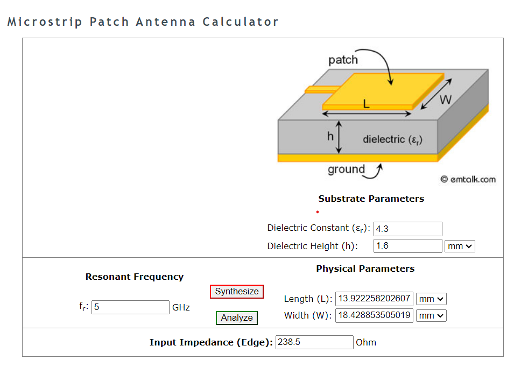
\includegraphics[width=.5\textwidth]{patchcalculator.png}
    \caption{Patch Calculator}
    \label{fig:patch_calculator}
\end{figure}


\textbf{Constant Values}
\begin{itemize}
    \item Height of the Conductor: 0.035 mm
    \item Height of the Substrate: 1.6 mm
    \item Width of the Feedline: 3.137 mm
    \item Height of Inset: 1mm
    \item Material for Ground and Patch: Copper (Annealed)
    \item Material for Substrate: FR-4 (Lossy)
\end{itemize}



These constant values provide a foundation for the designs, ensuring uniformity and adhering to industrial norms. The choice of materials, specifically copper for the ground and patch and FR-4 for the substrate, aligns with common industry practices for Microstrip patch antennas.

\vspace{10pt} % Add space above the image

\begin{figure}[H]
    \centering
    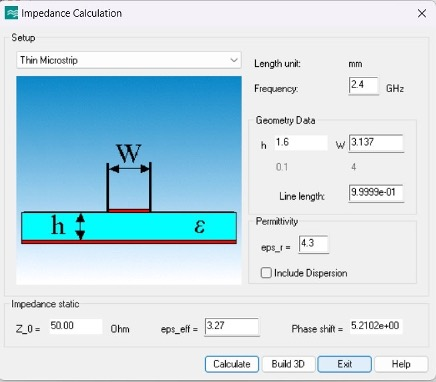
\includegraphics[width=0.5\textwidth]{widthcalculator.png}
    \caption{Calculation of Feedline Width}
    \label{fig:width_calculator}
\end{figure}

\vspace{10pt} % Add space below the image

The Transmission Line equations
\begin{itemize}
    \setlength\itemsep{0em} % Reduce space between items
    \item To Find Width (W)
    \begin{equation}
    	W = \frac{c}{2f_r \sqrt{\frac{\varepsilon_r + 1}{2}}}
    \end{equation}

    \item To find the effective dielectric constant
    \begin{equation}
        \varepsilon_{\text{eff}} = \frac{\varepsilon_r + 1}{2} + \frac{\varepsilon_r - 1}{2}\left(1 + 12 \frac{h}{W}\right)^{-\frac{1}{2}}
    \end{equation}

    \item To find the effective length
    \begin{equation}
        L_{\text{eff}} = \frac{c}{2f_r \sqrt{\varepsilon_{\text{eff}}}}
    \end{equation}
\end{itemize}




Online calculators were used to get rough values of Length and Width of Patch for design. Calculating width of Feedline using the in-built calculator in CST Microwave Studio. Even with the given formulas, the calculated parameters don’t often give us the desired result. Optimizing the antenna at desired frequencies involves iterative adjustments of the width and length, accompanied by different simulations of parameter sweeps of different parameters. These sweeps enabled us to visualize the performance metrics across a range of parameter values, ensuring optimal performance at the desired frequency.

Insets, strategically integrated gaps within the antenna structure, serve as a critical design element. They are employed to manipulate electrical properties and tailor the antenna's behavior. The variation in inset length is systematically explored, providing insights into its influence on the dip in the magnitude of the S parameters.

\begin{figure}[H]
    \centering
    \begin{minipage}{0.48\textwidth}
        \centering
        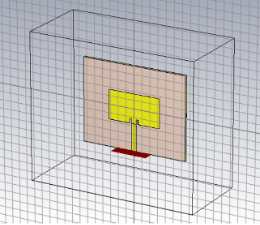
\includegraphics[width=\textwidth]{4inset1.png}
        \caption{Perspective View of 4 GHz Design }
        \label{fig:4ghz_inset1}
    \end{minipage}
    \hfill % this will insert a space between the two figures
    \begin{minipage}{0.48\textwidth}
        \centering
        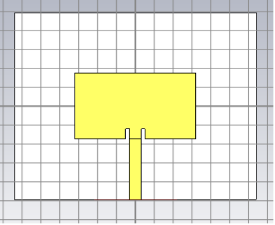
\includegraphics[width=\textwidth]{4inset2.png}
        \caption{Front View of 4 GHz Design}
        \label{fig:4ghz_inset2}
    \end{minipage}
\end{figure}

\begin{figure}[H]
    \centering
    \begin{minipage}{0.48\textwidth}
        \centering
        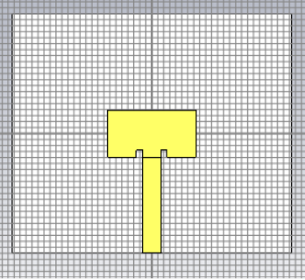
\includegraphics[width=\textwidth]{4inset3.png}
        \caption{Perspective View of 8 GHz Design}
        \label{fig:4ghz_inset3}
    \end{minipage}
    \hfill % this will insert a space between the two figures
    \begin{minipage}{0.48\textwidth}
        \centering
        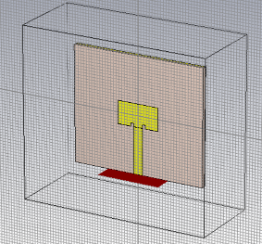
\includegraphics[width=\textwidth]{8inset1.png}
        \caption{Front View of 8 GHz Design}
        \label{fig:8ghz_inset1}
    \end{minipage}
\end{figure}



\subsection{Dataset Preparation and Antenna Simulation}

Simulations in CST Studio yield S parameter results for each antenna design. The meticulous focus is on collecting data for frequencies within the 1 to 10 GHz range, ensuring that the dip in magnitude is consistently less than -20 dB. This stringent criterion guarantees the inclusion of simulations representing antennas meeting the specified requirements.

\begin{figure}[H]
    \centering
    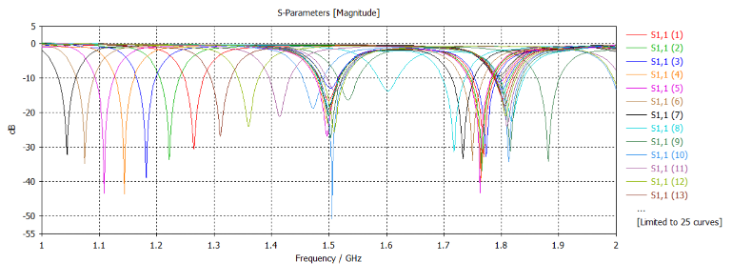
\includegraphics[width=0.8\textwidth]{s1to2.png}
    \caption{S parameters for different parameter values from a single design based on frequency range from 1 to 2 Ghz}
    \label{fig:s1to2}
\end{figure}

\begin{figure}[H]
    \centering
    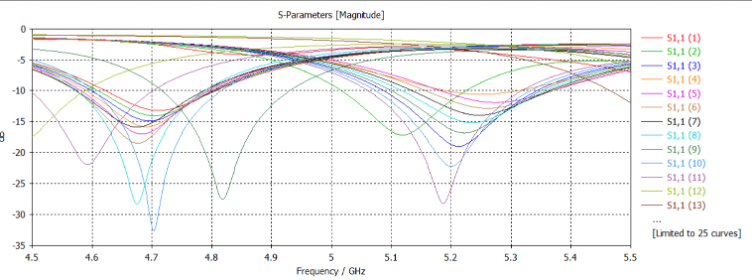
\includegraphics[width=0.8\textwidth]{s4to5.png}
    \caption{S parameters for different parameter values from a single design based on frequency range from 4.5 to 5.5 Ghz}
    \label{fig:s4to5}
\end{figure}




The overarching objective is to develop a machine learning module capable of predicting antenna parameters—length, width, and inset length—based on the frequency and magnitude of the S parameters. The dataset is structured to encompass input features such as frequency and magnitude, with corresponding outputs being the antenna parameters. The utilization of consistent values across designs provides a controlled environment for the study.

\begin{longtable}{|l|l|l|l|l|l|}
\caption{Detailed Antenna Parameters and Measurements} \label{tab:antenna_measurements} \\
\hline
\textbf{S.no} & \textbf{F (GHz)} & \textbf{L (mm)} & \textbf{W (mm)} & \textbf{b (mm)} & \textbf{Mag(db)} \\ \hline
\endfirsthead
\multicolumn{6}{c}%
{{\bfseries Table \thetable\ continued from previous page}} \\
\hline
\textbf{S.no} & \textbf{F (GHz)} & \textbf{L (mm)} & \textbf{W (mm)} & \textbf{b (mm)} & \textbf{Mag(db)} \\ \hline
\endhead
\hline
\endfoot
% All data rows
1 & 2.16 & 28.4 & 66.5 & 3 & -38.86 \\ \hline
2 & 2.113 & 28 & 68 & 3 & -20.3 \\ \hline
3 & 2.32 & 29 & 68 & 3 & -25.1 \\ \hline
4 & 2.165 & 29 & 66.5 & 6 & -22.9 \\ \hline
5 & 1.025 & 68 & 90 & 10 & -32 \\ \hline
6 & 1.1 & 63 & 90 & 6 & -39.4 \\ \hline
7 & 1.06 & 65 & 90 & 6 & -39.62 \\ \hline
8 & 1.085 & 64 & 90 & 6 & -42.3 \\ \hline
9 & 1.05 & 66 & 90 & 6 & -35.44 \\ \hline
10 & 1.024 & 68 & 86 & 6 & -28 \\ \hline
11 & 3 & 23 & 40 & 3 & -21.6 \\ \hline
12 & 1.814 & 46 & 78 & 8 & -42.5 \\ \hline
13 & 1.81 & 49 & 78 & 8 & -23.9 \\ \hline
14 & 4 & 16.87 & 30 & 3 & -42.4 \\ \hline
15 & 4.1 & 16.4 & 30 & 3 & -21.55 \\ \hline
16 & 3.94 & 17.2 & 30 & 3 & -30.8 \\ \hline
17 & 3.89 & 17.4 & 30 & 2.7 & -21.41 \\ \hline
18 & 3.88 & 17.4 & 32 & 2.7 & -28.3 \\ \hline
19 & 2.01 & 34 & 64 & 3 & -21.78 \\ \hline
20 & 1.81 & 38 & 64 & 3 & -32.3 \\ \hline
21 & 1.86 & 37 & 64 & 3 & -42.8 \\ \hline
22 & 1.9 & 36 & 64 & 3 & -36.18 \\ \hline
23 & 4.55 & 15 & 26 & 2.5 & -26.86 \\ \hline
24 & 4.56 & 15 & 25.5 & 2.5 & -21.42 \\ \hline
25 & 4.63 & 14.7 & 26 & 2.5 & -28.79 \\ \hline
26 & 4.71 & 14.4 & 26 & 2.5 & -25.2 \\ \hline
27 & 4.63 & 14.4 & 26 & 2.6 & -47.5 \\ \hline
28 & 2.12 & 28.4 & 68 & 7.5 & -29.84 \\ \hline
29 & 2.4 & 29 & 38 & 6 & -20.8 \\ \hline
30 & 1.265 & 55 & 78 & 8 & -30.55 \\ \hline
31 & 1.1 & 63 & 78 & 8 & -43.4 \\ \hline
32 & 1.22 & 57 & 78 & 8 & -33.5 \\ \hline
33 & 1.18 & 59 & 78 & 8 & -39 \\ \hline
34 & 1.14 & 61 & 78 & 8 & -43.6 \\ \hline
35 & 1.414 & 49 & 78 & 8 & -21.2 \\ \hline
36 & 1.36 & 51 & 78 & 8 & -23.98 \\ \hline
37 & 1.31 & 53 & 78 & 8 & -26.91 \\ \hline
38 & 1.5 & 46 & 80 & 6 & -20.56 \\ \hline
39 & 1.497 & 46 & 80 & 3 & -26.81 \\ \hline
40 & 1.5 & 46 & 70 & 8 & -25.5 \\ \hline
41 & 1.68 & 41 & 70 & 6 & -22.56 \\ \hline
42 & 1.6 & 43 & 70 & 6 & -28.7 \\ \hline
43 & 1.53 & 45 & 70 & 6 & -39.05 \\ \hline
44 & 1.86 & 37 & 64 & 5 & -23.43 \\ \hline
45 & 1.61 & 43 & 64 & 5 & -26 \\ \hline
46 & 5.2 & 13 & 21.5 & 2.5 & -22.24 \\ \hline
47 & 5.18 & 13 & 22 & 2.5 & -28.25 \\ \hline
48 & 4.67 & 14.5 & 24 & 3 & -28.33 \\ \hline
49 & 4.818 & 14 & 24 & 3 & -27.56 \\ \hline
50 & 4.7 & 14.4 & 24 & 3 & -32.65 \\ \hline
51 & 4.59 & 14.8 & 24 & 3 & -21.95 \\ \hline
52 & 4.67 & 13.5 & 22 & 2.5 & -28.33 \\ \hline
53 & 5.15 & 13.1 & 22 & 2.5 & -25.26 \\ \hline
54 & 5.12 & 13.2 & 22 & 2.5 & -23.2 \\ \hline
55 & 5.05 & 13.4 & 22 & 2.5 & -20.29 \\ \hline
56 & 5.034 & 13.4 & 22 & 3 & -44.8 \\ \hline
57 & 5 & 13.55 & 22 & 3 & -32.43 \\ \hline
58 & 4.95 & 13.7 & 22 & 3 & -26.98 \\ \hline
59 & 4.9 & 13.85 & 22 & 3 & -23.54 \\ \hline
60 & 5.367 & 12.5 & 21 & 3 & -23 \\ \hline
61 & 5.485 & 12.2 & 20.6 & 3 & -20.38 \\ \hline
62 & 5.45 & 12.3 & 20.6 & 3 & -22.55 \\ \hline
63 & 5.41 & 12.4 & 20.6 & 3 & -25.2 \\ \hline
64 & 5.34 & 12.6 & 20.6 & 3 & -34.59 \\ \hline
65 & 6.05 & 10.5 & 33 & 1.6 & -31.21 \\ \hline
66 & 6.315 & 10 & 33 & 1.6 & -21.76 \\ \hline
67 & 6.26 & 10.1 & 33 & 1.6 & -23.047 \\ \hline
68 & 6.21 & 10.2 & 33 & 1.6 & -24.5 \\ \hline
69 & 6.1 & 10.4 & 33 & 1.6 & -28.42 \\ \hline
70 & 5.975 & 10.7 & 33 & 1.6 & -40.1 \\ \hline
71 & 5.88 & 10.9 & 33 & 1.6 & -39.8 \\ \hline
72 & 5.83 & 11 & 33 & 1.6 & -33.98 \\ \hline
73 & 7.82 & 8.4 & 15.4 & 1.2 & -37.78 \\ \hline
74 & 7.79 & 8.4 & 15.6 & 1.2 & -25.85 \\ \hline
75 & 7.68 & 8.6 & 15.6 & 1.2 & -26.58 \\ \hline
76 & 7.62 & 8.7 & 15.4 & 1.2 & -20.37 \\ \hline
77 & 8.16 & 8 & 14.8 & 1.2 & -23.1 \\ \hline
78 & 8.22 & 7.9 & 14.7 & 1.2 & -21.28 \\ \hline
79 & 10.44 & 6.5 & 9.2 & 1.8 & -42.9 \\ \hline
80 & 10.34 & 6.6 & 9.2 & 1.8 & -25.94 \\ \hline
81 & 9.78 & 7 & 9.7 & 1.9 & -24.13 \\ \hline
82 & 9.97 & 6.8 & 9.7 & 1.9 & -33.68 \\ \hline
83 & 9.88 & 6.9 & 9.7 & 1.9 & -33.1 \\ \hline
84 & 9.7 & 7.1 & 9.7 & 1.9 & -20 \\ \hline
85 & 9.57 & 7.2 & 9.7 & 2 & -21.8 \\ \hline
86 & 9.353 & 7.4 & 9.7 & 2.1 & -20 \\ \hline
87 & 9.23 & 7.5 & 9.7 & 2.2 & -21.98 \\ \hline
88 & 9.16 & 7.5 & 10 & 2.2 & -28.94 \\ \hline
89 & 8.95 & 7.7 & 10.2 & 2.2 & -21.62 \\ \hline
\end{longtable}


\section{Machine Learning Model Tuning}
\label{sec:preparing_dataset_and_fitting_model}

\subsection{Dataset Compilation}
The dataset, crucial for the ML model, was compiled from a range of simulations. This data is instrumental in training the machine learning model to predict optimal antenna parameters. 

\subsection{Model Selection}
The RandomForestRegressor was chosen due to its robustness and effectiveness in handling regression tasks with high-dimensional data, characteristic of electromagnetic design problems.

\subsection{Data Preparation}
The dataset was loaded into a pandas DataFrame, a flexible and powerful data manipulation tool for Python, allowing for easy data analysis and manipulation. The dataset consists of input features such as the frequency and magnitude of the S parameters, with the target variables being the length (L), width (W), and inset length (b) of the antenna.

\subsubsection{Splitting the Data}
A key step in machine learning model preparation is splitting the dataset into training and testing sets. This is crucial for evaluating the model's performance on unseen data. The standard practice of an 80-20 split provides a substantial amount of data for training while reserving enough for an unbiased assessment of the model's generalization capabilities.

\subsection{Model Training}
The RandomForestRegressor model, a collection of decision trees, is known for its high accuracy and ability to run in parallel. It's an ensemble method that fits multiple decision tree classifiers on various sub-samples of the dataset and averages the results to improve predictive accuracy and control over-fitting.

\subsubsection{Performance Evaluation}
Training the model involves adjusting the decision trees to best fit the training data. The Mean Squared Error (MSE) metric is used post-training on the test set to quantify the model's prediction accuracy.

\subsection{Model Evaluation and Visualization}
Visualizations of the actual versus predicted values offer an intuitive understanding of the model's performance. The proximity of the predicted points to the actual points indicates the level of precision achieved by the RandomForestRegressor model.

\subsection{Code Implementation}
The code snippets demonstrate the process using Python's machine learning library, scikit-learn.

\begin{verbatim}
import pandas as pd
from sklearn.model_selection import train_test_split
from sklearn.ensemble import RandomForestRegressor
from sklearn.metrics import mean_squared_error

# Load the dataset
file_path = 'Dataset_inset.xlsx'
df = pd.read_excel(file_path)

# Separate data into features (X) and target variables (y)
X_rev = df[['F', 'Mag(db)']]
y_rev = df[['L', 'W', 'b']]

# Split the data into training and testing sets (80% train, 20% test)
X_rev_train, X_rev_test, y_rev_train, y_rev_test = train_test_split(X_rev, y_rev, test_size=0.2, random_state=42)

# Train Random Forest models
model_rev = RandomForestRegressor(n_estimators=100, random_state=42)
model_rev.fit(X_rev_train, y_rev_train)

# Make predictions on the test set
y_rev_pred = model_rev.predict(X_rev_test)

# Evaluate the model
mse_rev = mean_squared_error(y_rev_test, y_rev_pred)
print(f'Mean Squared Error for L, W, b: {mse_rev}')
\end{verbatim}





\section{Simulating Antennas on Predicted Values}
\label{sec:exploring_other_techniques}
Insets play a pivotal role in influencing impedance matching, bandwidth, and radiation patterns, offering additional degrees of freedom for design optimization...


\begin{table}
   \caption{Predicted Antenna Dimensions v/s Actual Values}
    \small % Reduce font size
    \centering
    \begin{tabular}{|l|l|l|l|l|l|l|l|}
    \hline
    \textbf{F} & \textbf{Mag(db)} & \textbf{Actual\_L} & \textbf{Predicted\_L} & \textbf{Actual\_W} & \textbf{Predicted\_W} & \textbf{Actual\_b} & \textbf{Predicted\_b} \\ \hline
    1.5 & -20.56 & 46 & 45.66 & 80 & 72.86 & 6 & 6.95 \\ \hline
    1.81 & -32.3 & 38 & 45.71 & 64 & 74.52 & 3 & 6.6 \\ \hline
    5.15 & -25.26 & 13.1 & 13.30 & 22 & 21.91 & 2.5 & 2.67 \\ \hline
    5.975 & -40.1 & 10.7 & 10.83 & 33 & 32.88 & 1.6 & 1.61 \\ \hline
    2.16 & -38.86 & 28.4 & 28.97 & 66.5 & 67.54 & 3 & 6.3 \\ \hline
    4.56 & -21.42 & 15 & 15.00 & 25.5 & 25.3 & 2.5 & 2.76 \\ \hline
    1.31 & -26.91 & 53 & 53.11 & 78 & 78.18 & 8 & 7.43 \\ \hline
    6.05 & -31.21 & 10.5 & 10.60 & 33 & 32.75 & 1.6 & 1.63 \\ \hline
    1.085 & -42.3 & 64 & 63.15 & 90 & 82.08 & 6 & 7.32 \\ \hline
    1.6 & -28.7 & 43 & 43.98 & 70 & 67.64 & 6 & 5.3 \\ \hline
    9.78 & -24.13 & 7 & 7.08 & 9.7 & 9.68 & 1.9 & 1.93 \\ \hline
    1.18 & -39 & 59 & 61.05 & 78 & 81.24 & 8 & 7.46 \\ \hline
    9.23 & -21.98 & 7.5 & 7.50 & 9.7 & 9.95 & 2.2 & 2.15 \\ \hline
    5.367 & -23 & 12.5 & 12.48 & 21 & 20.68 & 3 & 2.97 \\ \hline
    1.024 & -28 & 68 & 66.53 & 86 & 89.28 & 6 & 8.68 \\ \hline
    2.113 & -20.3 & 28 & 29.07 & 68 & 67.16 & 3 & 4.46 \\ \hline
    3.94 & -30.8 & 17.2 & 17.21 & 30 & 30.53 & 3 & 2.77 \\ \hline
    4.71 & -25.2 & 14.4 & 14.13 & 26 & 23.58 & 2.5 & 2.88 \\ \hline
    5.18 & -28.25 & 13 & 13.24 & 22 & 21.80 & 2.5 & 2.68 \\ \hline
    \end{tabular}
\end{table}

\begin{figure}[H]
    \centering
    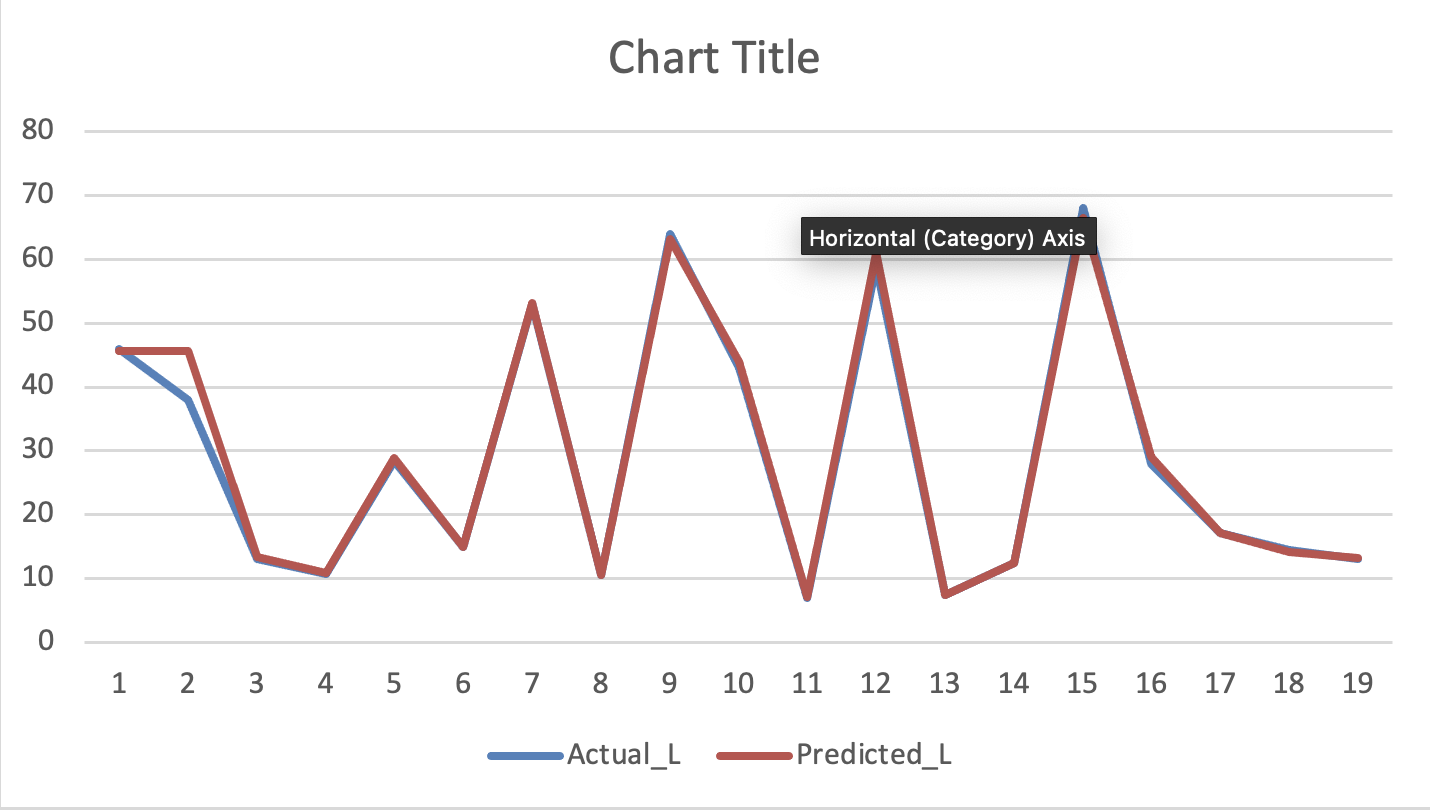
\includegraphics[width=0.8\textwidth]{1.png}
    \caption{Predicted Length v/s Actual Length}
    \label{fig:s1to2}
\end{figure}
\begin{figure}[H]
    \centering
    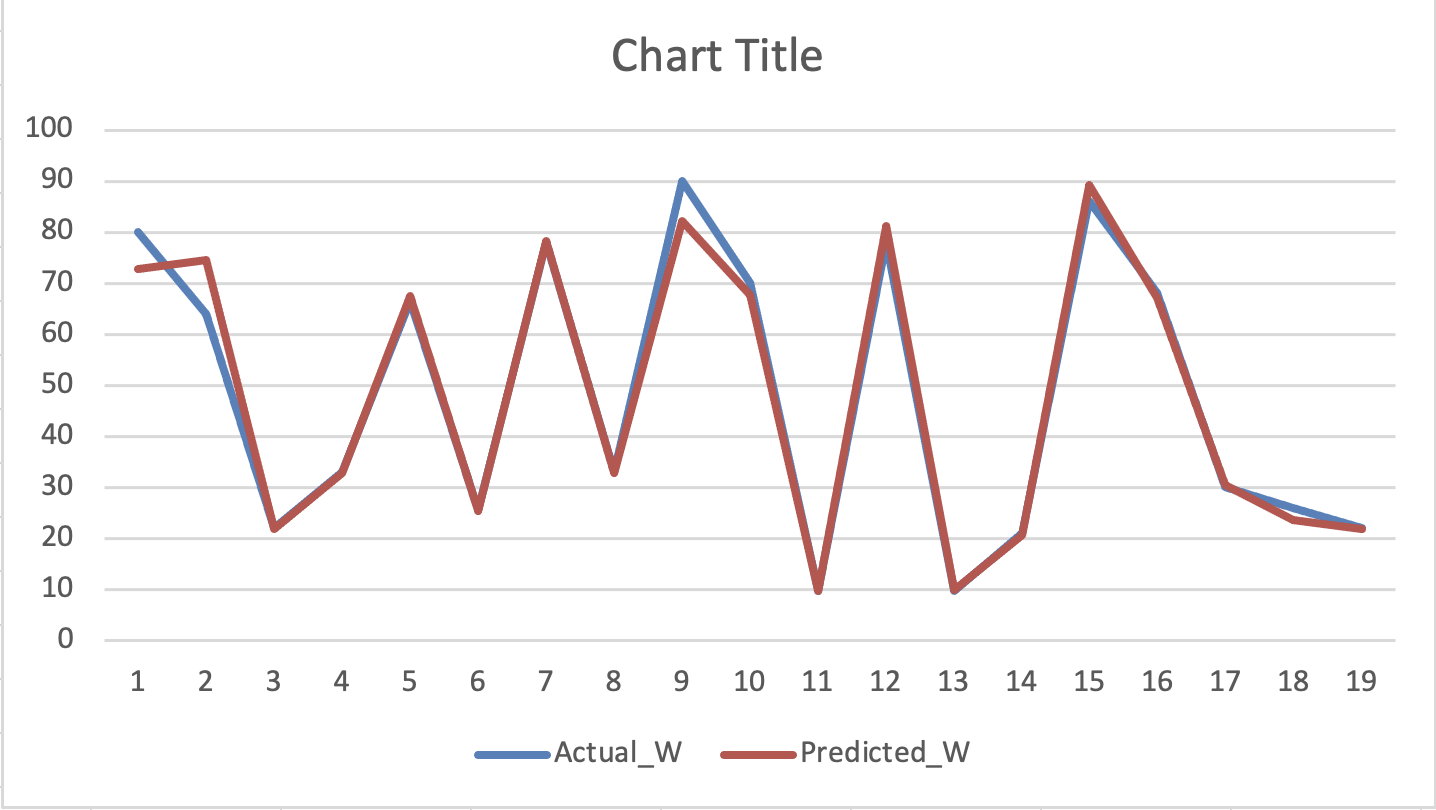
\includegraphics[width=0.8\textwidth]{2.png}
    \caption{Predicted Width v/s Actual Width}
    \label{fig:s1to2}
\end{figure}
\begin{figure}[H]
    \centering
    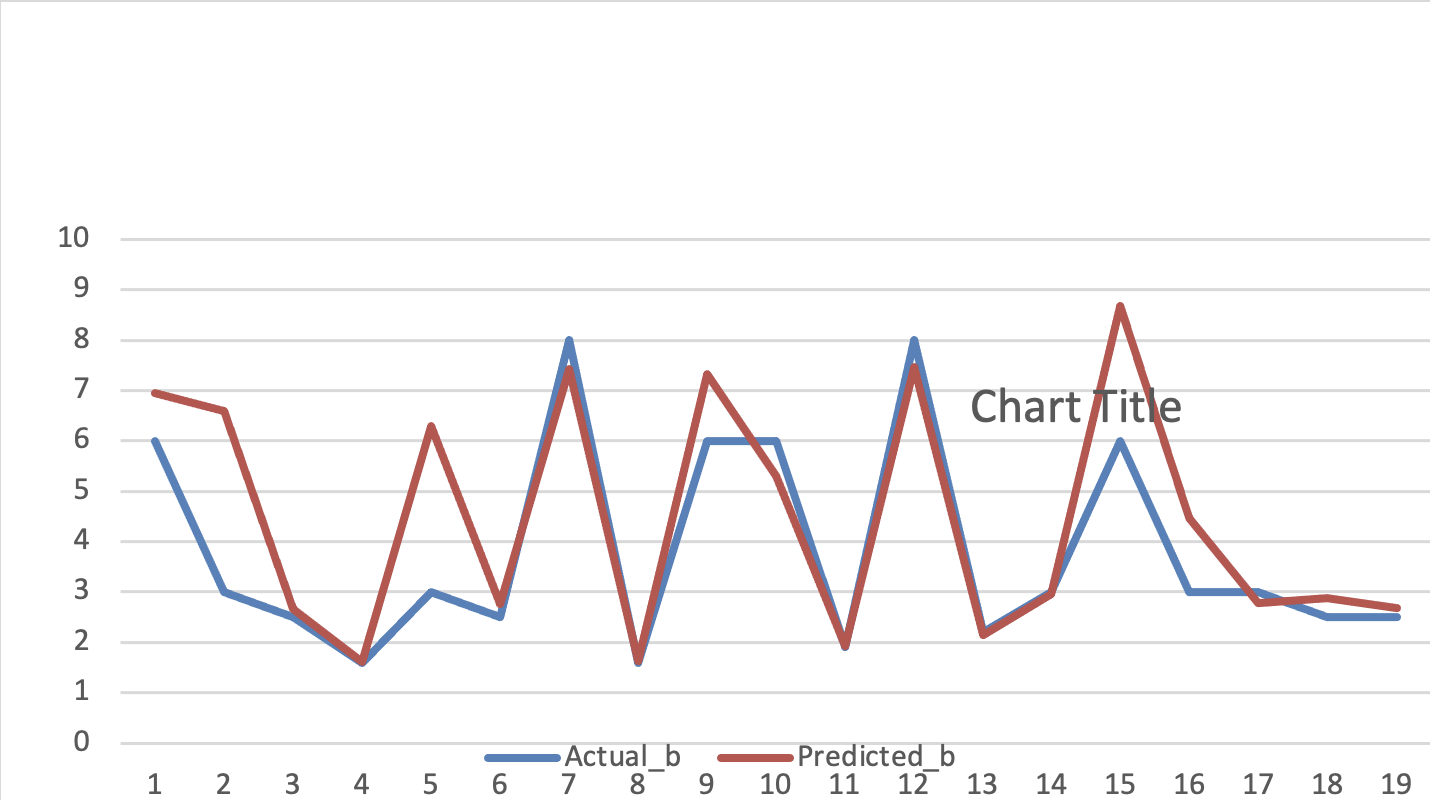
\includegraphics[width=0.8\textwidth]{3.png}
    \caption{Predicted Inset Height v/s Actual Height}
    \label{fig:s1to2}
\end{figure}


\begin{figure}[H]
    \centering
    \begin{minipage}{0.48\textwidth}
        \centering
        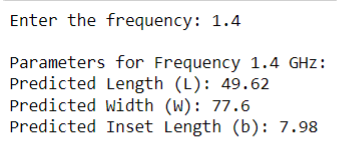
\includegraphics[width=\textwidth,height =5cm]{data14.png}
        \caption{Parameters predicted for 1.4 GHz}
        \label{fig:4ghz_inset1}
    \end{minipage}
    \hfill % this will insert a space between the two figures
    \begin{minipage}{0.48\textwidth}
        \centering
        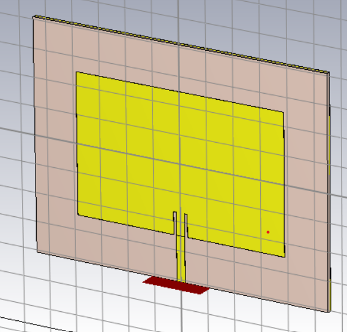
\includegraphics[width=\textwidth,height =5cm]{pred14img.png}
        \caption{Design from Predicted Parameters (1.4 GHz)}
        \label{fig:4ghz_inset2}
    \end{minipage}
\end{figure}
\begin{figure}[H]
    \centering
    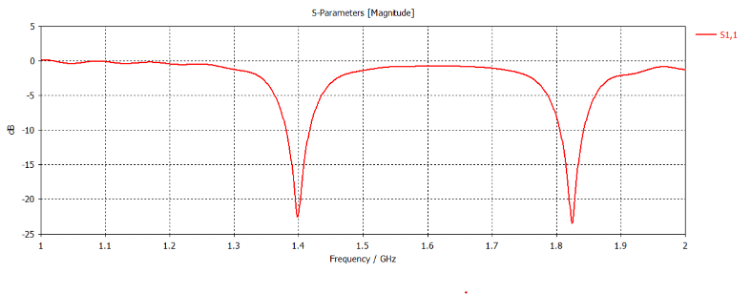
\includegraphics[width=0.8\textwidth]{pred14.png}
    \caption{S Parameters dipping at 1.4GHz}
    \label{fig:width_calculator}
\end{figure}


\begin{figure}[H]
    \centering
    \begin{minipage}{0.48\textwidth}
        \centering
        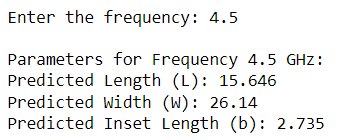
\includegraphics[width=\textwidth,height =5cm]{data45.png}
        \caption{Parameters predicted for 4.5 GHz}
        \label{fig:4ghz_inset1}
    \end{minipage}
    \hfill % this will insert a space between the two figures
    \begin{minipage}{0.48\textwidth}
        \centering
        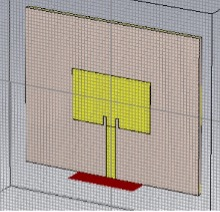
\includegraphics[width=\textwidth,height =5cm]{pred45im.png}
        \caption{Design from Predicted Parameters (4.5 GHz)}
        \label{fig:4ghz_inset2}
    \end{minipage}
\end{figure}
\begin{figure}[H]
    \centering
    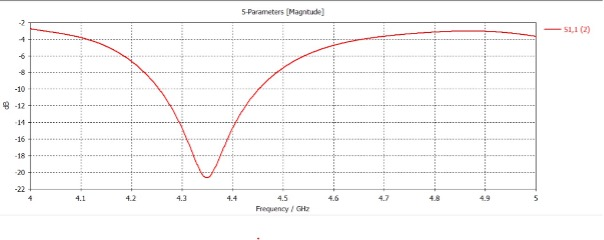
\includegraphics[width=0.8\textwidth]{pred45.jpg}
    \caption{S Parameters dipping at 4.35GHz (Error of -0.15GHz)}
    \label{fig:width_calculator}
\end{figure}




\begin{figure}[H]
    \centering
    \begin{minipage}{0.48\textwidth}
        \centering
        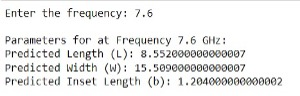
\includegraphics[width=\textwidth,height =5cm]{data76.png}
        \caption{Parameters predicted for 7.6 GHz}
        \label{fig:4ghz_inset1}
    \end{minipage}
    \hfill % this will insert a space between the two figures
    \begin{minipage}{0.48\textwidth}
        \centering
        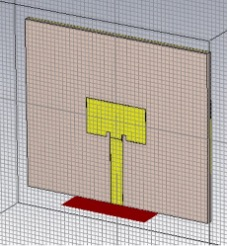
\includegraphics[width=\textwidth,height =5cm]{pred76img.png}
        \caption{Design from Predicted Parameters (7.6 GHz)}
        \label{fig:4ghz_inset2}
    \end{minipage}
\end{figure}
\begin{figure}[H]
    \centering
    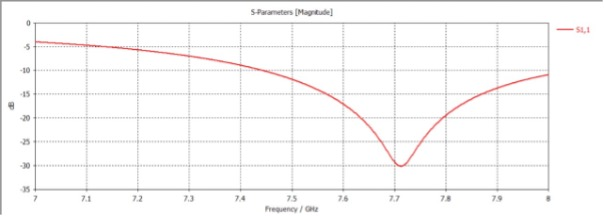
\includegraphics[width=0.8\textwidth]{pred76.jpg}
    \caption{S Parameters dipping at 7.71GHz (Error of 0.11GHz)}
    \label{fig:width_calculator}
\end{figure}

\begin{figure}[H]
    \centering
    \begin{minipage}{0.48\textwidth}
        \centering
        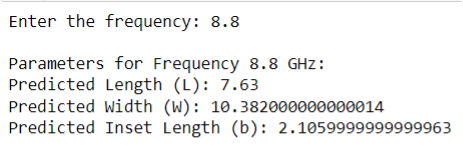
\includegraphics[width=\textwidth,height =5cm]{data88.png}
        \caption{Parameters predicted for 8.8 GHz}
        \label{fig:4ghz_inset1}
    \end{minipage}
    \hfill % this will insert a space between the two figures
    \begin{minipage}{0.48\textwidth}
        \centering
        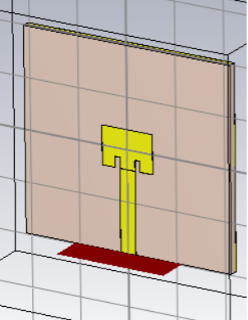
\includegraphics[width=\textwidth,height =5cm]{pred88img.png}
        \caption{Design from Predicted Parameters (8.8 GHz)}
        \label{fig:4ghz_inset2}
    \end{minipage}
\end{figure}
\begin{figure}[H]
    \centering
    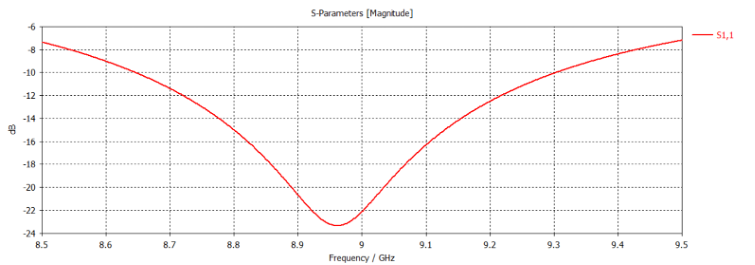
\includegraphics[width=0.8\textwidth]{pred88.png}
    \caption{S Parameters dipping at 8.96GHz (Error of 0.16GHz)}
    \label{fig:width_calculator}
\end{figure}

\subsection{Limitations}
In our study, we have identified several limitations that are important to consider when using the machine learning model for design optimization:

\begin{enumerate}
    \item \textbf{Limited Dataset Size:} The performance of the current model is contingent on the size and diversity of the dataset. A larger and more diverse dataset would likely enhance the model's ability to generalize. The long simulation time in CST Studio slows down the process for data collection, making it a very redundant and time-consuming process.

    \item \textbf{Assumption of Linearity:} Random Forest models assume a certain level of linearity in relationships. If the relationships between antenna parameters are highly non-linear, the model may not capture them effectively. Consequently, this contributes to the observation that the length of the patch tends to be predicted more accurately, on average, in comparison to the height of the inset gap. The latter parameter exhibits a less linear relationship with antenna frequencies, especially at close frequency levels.

    \item \textbf{Interpretability:} Random Forest models, while effective, can be challenging to interpret. Understanding the exact decision-making process of the model may be complex.

    \item \textbf{Extrapolation Challenges:} The model may struggle with accurate predictions for frequencies or magnitudes outside the range of the training data. Care must be taken when extrapolating predictions. Hence, our model mostly works well only for frequencies ranging between 1 to 10 GHz.
\end{enumerate}




\section{Online Dashboard and Public Repository}
\label{sec:final_comparison_and_shortcomings}

To promote collaboration and accessibility, we have established an online dashboard for our research and dataset. You can explore our work and interact with the dataset at \url{https://ml-antenna-design.streamlit.app/}.

This dashboard offers a user-friendly interface for researchers and enthusiasts to delve into our findings, experiment with the dataset, and contribute to further improvements.
Furthermore, we have made our dataset and machine learning model openly available on GitHub at \url{https://github.com/akshatpunia26/optimal-antenna-design/}. Our repository is designed to encourage contributions from the community, allowing researchers to access, analyze, and build upon our work. We welcome collaborative efforts to enhance the capabilities of our antenna design model.

The focus of our dataset collection has been on frequencies within the 1 to 10 GHz range, ensuring a consistent magnitude dip of less than -20 dB.

\begin{figure}[H]
    \centering
    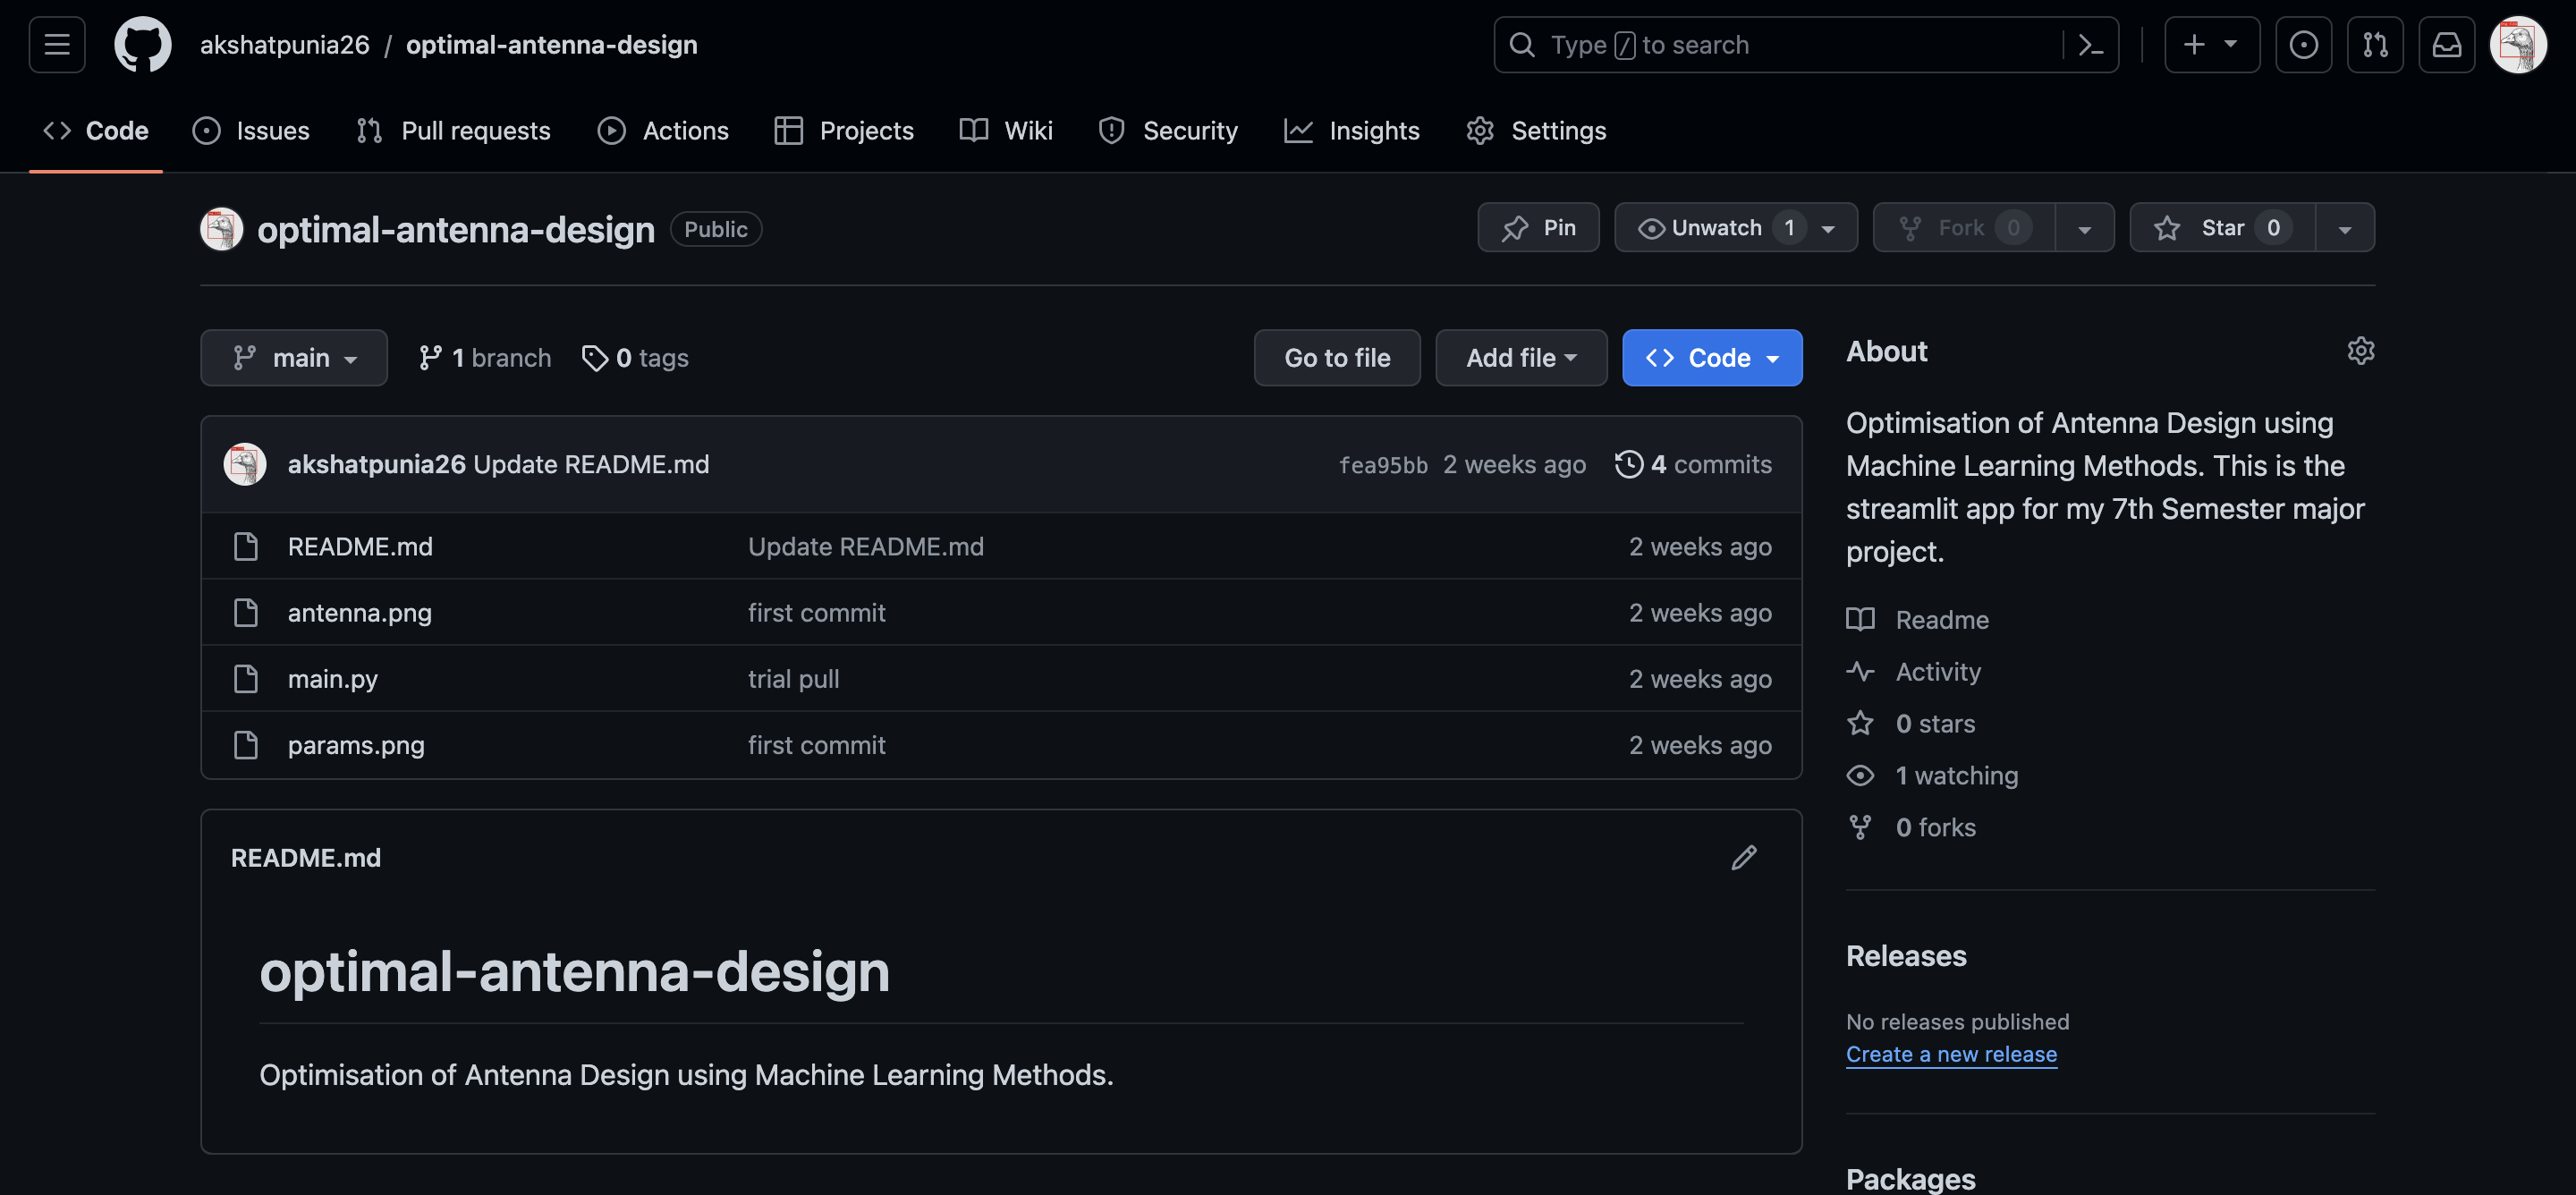
\includegraphics[width=1\textwidth]{github.png}
    \label{fig:width_calculator}
\end{figure}



\chapter{Conclusion}
In conclusion, the integration of machine learning (ML) techniques into the field of antenna design has proven to be a feasible and promising endeavor. The predictive models generated through ML have demonstrated a notable closeness to the desired design parameters, significantly reducing the time and effort required for iterative design processes. 
\linebreak
\par The dataset produced by the electromagnetic simulator CST Microwave Studio serves as a valuable foundation for future studies and paves the way for the integration of more advanced ML techniques and models. This innovative approach holds great potential for revolutionizing antenna design processes, making them more efficient and adaptable to various real-world applications. As we move forward, further research and development in this direction will undoubtedly yield even more remarkable results, pushing the boundaries of what is achievable in the field of electromagnetic design.


\chapter{Future Prospects}

In the future we plan to implement the following changes. :

\begin{enumerate}
    \item \textbf{More Diverse Dataset:}
    \begin{itemize}
        \item \textit{Expand Antenna Types:} The dataset can be expanded to include data from a variety of antenna types beyond Rectangular Microstrip Patch Antennas. This could encompass designs such as circular patches, triangular patches, and other non-rectangular geometries, each with unique parameter dependencies.
        \item \textit{Frequency Bands:} We aim to  cover a broader spectrum of frequency bands. Different frequency bands may exhibit distinct behaviors, and the model could benefit from exposure to this extensive range.
        \item \textit{Real World Constraints:} Introducing real-world constraints into the dataset, such as manufacturing tolerances, material imperfections, or environmental factors, will make the model more robust and applicable to practical scenarios.
    \end{itemize}

    \item \textbf{Deep Learning Models:} There is a plan to implement deep learning models, specifically neural networks, to capture the complex non-linear relationships in the data. Neural networks have the ability to automatically learn hierarchical representations from the input features, which could prove beneficial for the model's predictive capability.

    \item \textbf{Continuous Model Updating:} A system for continuous model updating will be put in place as more data becomes available. This will ensure that the model remains up-to-date and adapts to new antenna design patterns and technological advancements.

    \item \textbf{Real-World Development and Integration with Design Tools:}
    \begin{itemize}
        \item The integration of the trained model into a real-world antenna design workflow is being explored. A user-friendly interface for engineers to input parameters and receive predicted antenna dimensions could significantly streamline the design process.
        \item Efforts are underway to explore integration with popular antenna design tools. This could facilitate the automated extraction of design parameters and contribute to the dataset during the design process, creating a feedback loop that continuously improves the model's accuracy and reliability.
    \end{itemize}
\end{enumerate}

These advancements are envisioned to not only improve the precision of antenna design predictions but also to bridge the gap between theoretical models and practical, real-world applications. The future looks promising for the field of antenna design optimization, with machine learning at the forefront of this innovative journey.


\pagebreak

\addcontentsline{toc}{chapter}{Bibliography}
\begin{thebibliography}{99}
\bibitem{lecci2020}
M. Lecci, P. Testolina, M. Rebato, A. Testolin, and M. Zorzi,
\newblock ``Machine Learning-aided Design of Thinned Antenna Arrays for Optimized Network Level Performance,''
\newblock 14th European Conference on Antennas and Propagation (EuCAP 2020), Copenhagen, 2020.

\bibitem{liu}
Bo Liu, Hadi Aliakbarian, Zhongkun Ma, Guy A. E. Vandenbosch, Georges Gielen, and Peter Excell,
\newblock ``An Efficient Method for Antenna Design Optimization Based on Evolutionary Computation and Machine Learning Techniques.''

\bibitem{misilmani2018}
Hilal M. El Misilmani, Tarek Naous, and Salwa K. Al Khatib,
\newblock ``A review on the design and optimization of antennas using machine learning algorithms and techniques,''
\newblock Advances in Science, Technology and Engineering Systems Journal, Vol. 3, No. 5, 394-397, 2018.

\bibitem{gangwar2008}
Som Pal Gangwar, R. P. S. Gangwar, B. K. Kanaujia, and Paras,
\newblock ``Resonant frequency of circular microstrip antenna using artificial neural networks,''
\newblock Indian Journal of Radio & Space Physics, Vol. 37, June 2008.

\bibitem{jain}
Satish K. Jain, Amalendu Patnaik, and Sachendra N. Sinha,
\newblock ``Design of custom-made stacked patch antennas: a machine learning approach,''
\newblock International Journal of Machine Learning & Cybernetics.

\bibitem{kushwah}
Vivek Singh Kushwah and Geetam Singh Tomar,
\newblock ``Design and Analysis of Microstrip Patch Antennas Using Artificial Neural Network.''


\end{thebibliography}

\end{document}